\documentclass[10pt,a4paper]{article}

\usepackage[spanish,activeacute,es-tabla]{babel}
\usepackage[utf8]{inputenc}
\usepackage{ifthen}
\usepackage{listings}
\usepackage{dsfont}
\usepackage{subcaption}
\usepackage{amsmath}
\usepackage[strict]{changepage}
\usepackage[top=1cm,bottom=2cm,left=1cm,right=1cm]{geometry}%
\usepackage{color}%
\newcommand{\tocarEspacios}{%
	\addtolength{\leftskip}{3em}%
	\setlength{\parindent}{0em}%
}

% Especificacion de procs

\newcommand{\In}{\textsf{in }}
\newcommand{\Out}{\textsf{out }}
\newcommand{\Inout}{\textsf{inout }}

\newcommand{\encabezadoDeProc}[4]{%
	% Ponemos la palabrita problema en tt
	%  \noindent%
	{\normalfont\bfseries\ttfamily proc}%
	% Ponemos el nombre del problema
	\ %
	{\normalfont\ttfamily #2}%
	\
	% Ponemos los parametros
	(#3)%
	\ifthenelse{\equal{#4}{}}{}{%
		% Por ultimo, va el tipo del resultado
		\ : #4}
}

\newenvironment{proc}[4][res]{%
	
	% El parametro 1 (opcional) es el nombre del resultado
	% El parametro 2 es el nombre del problema
	% El parametro 3 son los parametros
	% El parametro 4 es el tipo del resultado
	% Preambulo del ambiente problema
	% Tenemos que definir los comandos requiere, asegura, modifica y aux
	\newcommand{\requiere}[2][]{%
		{\normalfont\bfseries\ttfamily requiere}%
		\ifthenelse{\equal{##1}{}}{}{\ {\normalfont\ttfamily ##1} :}\ %
		\{\ensuremath{##2}\}%
		{\normalfont\bfseries\,\par}%
	}
	\newcommand{\asegura}[2][]{%
		{\normalfont\bfseries\ttfamily asegura}%
		\ifthenelse{\equal{##1}{}}{}{\ {\normalfont\ttfamily ##1} :}\
		\{\ensuremath{##2}\}%
		{\normalfont\bfseries\,\par}%
	}
	\renewcommand{\aux}[4]{%
		{\normalfont\bfseries\ttfamily aux\ }%
		{\normalfont\ttfamily ##1}%
		\ifthenelse{\equal{##2}{}}{}{\ (##2)}\ : ##3\, = \ensuremath{##4}%
		{\normalfont\bfseries\,;\par}%
	}
	\renewcommand{\pred}[3]{%
		{\normalfont\bfseries\ttfamily pred }%
		{\normalfont\ttfamily ##1}%
		\ifthenelse{\equal{##2}{}}{}{\ (##2) }%
		\{%
		\begin{adjustwidth}{+5em}{}
			\ensuremath{##3}
		\end{adjustwidth}
		\}%
		{\normalfont\bfseries\,\par}%
	}
	
	\newcommand{\res}{#1}
	\vspace{1ex}
	\noindent
	\encabezadoDeProc{#1}{#2}{#3}{#4}
	% Abrimos la llave
	\par%
	\tocarEspacios
}
{
	% Cerramos la llave
	\vspace{1ex}
}

\newcommand{\aux}[4]{%
	{\normalfont\bfseries\ttfamily\noindent aux\ }%
	{\normalfont\ttfamily #1}%
	\ifthenelse{\equal{#2}{}}{}{\ (#2)}\ : #3\, = \ensuremath{#4}%
	{\normalfont\bfseries\,;\par}%
}

\newcommand{\pred}[3]{%
	{\normalfont\bfseries\ttfamily\noindent pred }%
	{\normalfont\ttfamily #1}%
	\ifthenelse{\equal{#2}{}}{}{\ (#2) }%
	\{%
	\begin{adjustwidth}{+2em}{}
		\ensuremath{#3}
	\end{adjustwidth}
	\}%
	{\normalfont\bfseries\,\par}%
}

% Tipos

\newcommand{\nat}{\ensuremath{\mathds{N}}}
\newcommand{\ent}{\ensuremath{\mathds{Z}}}
\newcommand{\float}{\ensuremath{\mathds{R}}}
\newcommand{\bool}{\ensuremath{\mathsf{Bool}}}
\newcommand{\cha}{\ensuremath{\mathsf{Char}}}
\newcommand{\str}{\ensuremath{\mathsf{String}}}

% Logica

\newcommand{\True}{\ensuremath{\mathrm{true}}}
\newcommand{\False}{\ensuremath{\mathrm{false}}}
\newcommand{\Then}{\ensuremath{\rightarrow}}
\newcommand{\Iff}{\ensuremath{\leftrightarrow}}
\newcommand{\implica}{\ensuremath{\longrightarrow}}
\newcommand{\IfThenElse}[3]{\ensuremath{\mathsf{if}\ #1\ \mathsf{then}\ #2\ \mathsf{else}\ #3\ \mathsf{fi}}}
\newcommand{\yLuego}{\land _L}
\newcommand{\oLuego}{\lor _L}
\newcommand{\implicaLuego}{\implica _L}

\newcommand{\cuantificador}[5]{%
	\ensuremath{(#2 #3: #4)\ (%
		\ifthenelse{\equal{#1}{unalinea}}{
			#5
		}{
			$ % exiting math mode
			\begin{adjustwidth}{+2em}{}
				$#5$%
			\end{adjustwidth}%
			$ % entering math mode
		}
		)}
}

\newcommand{\existe}[4][]{%
	\cuantificador{#1}{\exists}{#2}{#3}{#4}
}
\newcommand{\paraTodo}[4][]{%
	\cuantificador{#1}{\forall}{#2}{#3}{#4}
}

%listas

\newcommand{\TLista}[1]{\ensuremath{seq \langle #1\rangle}}
\newcommand{\lvacia}{\ensuremath{[\ ]}}
\newcommand{\lv}{\ensuremath{[\ ]}}
\newcommand{\longitud}[1]{\ensuremath{|#1|}}
\newcommand{\cons}[1]{\ensuremath{\mathsf{addFirst}}(#1)}
\newcommand{\indice}[1]{\ensuremath{\mathsf{indice}}(#1)}
\newcommand{\conc}[1]{\ensuremath{\mathsf{concat}}(#1)}
\newcommand{\cab}[1]{\ensuremath{\mathsf{head}}(#1)}
\newcommand{\cola}[1]{\ensuremath{\mathsf{tail}}(#1)}
\newcommand{\sub}[1]{\ensuremath{\mathsf{subseq}}(#1)}
\newcommand{\en}[1]{\ensuremath{\mathsf{en}}(#1)}
\newcommand{\cuenta}[2]{\mathsf{cuenta}\ensuremath{(#1, #2)}}
\newcommand{\suma}[1]{\mathsf{suma}(#1)}
\newcommand{\twodots}{\ensuremath{\mathrm{..}}}
\newcommand{\masmas}{\ensuremath{++}}
\newcommand{\matriz}[1]{\TLista{\TLista{#1}}}
\newcommand{\seqchar}{\TLista{\cha}}

\renewcommand{\lstlistingname}{Código}
\lstset{% general command to set parameter(s)
	language=Java,
	morekeywords={endif, endwhile, skip},
	basewidth={0.47em,0.40em},
	columns=fixed, fontadjust, resetmargins, xrightmargin=5pt, xleftmargin=15pt,
	flexiblecolumns=false, tabsize=4, breaklines, breakatwhitespace=false, extendedchars=true,
	numbers=left, numberstyle=\tiny, stepnumber=1, numbersep=9pt,
	frame=l, framesep=3pt,
	captionpos=b,
}

\usepackage{caratula} % Version modificada para usar las macros de algo1 de ~> https://github.com/bcardiff/dc-tex


\titulo{Trabajo Práctico 1: Especificación y WP}
\subtitulo{"En Búsqueda del Camino"}

\fecha{\today}

\materia{Algoritmos y Estructuras de Datos}
\grupo{Grupo puntoJava}

\integrante{Gremes, Juan Ignacio}{21/24}{juanigremes@gmail.com}
\integrante{Anllo, Franciasco}{002/01}{email2@dominio.com}
\integrante{Naddeo, Matias}{651/24}{email3@dominio.com}
\integrante{Gutierrez, Marco}{167/24}{marcoantonio-gutierrez02@hotmail.com}

% Declaramos donde van a estar las figuras
% No es obligatorio, pero suele ser comodo
\graphicspath{{../static/}}

\begin{document}

\maketitle
%------------------------------- Empieza la seccion especificacion
\section{Especificación}


%                                            EJERCICIO 1.1
\subsection{grandesCiudades:}

A partir de una lista de ciudades, devuelve aquellas que tienen más de 50.000 habitantes.\\

\begin{proc}{grandesCiudades}{\In ciudades : \TLista{\str\times\ent}}{\TLista{\str\times\ent}}
	\requiere{True}
	\asegura{\paraTodo[unalinea]{i}{\ent}{(0 \leq i < |res|) \implicaLuego ((res[i] \in ciudades) \yLuego (res[i]_1 > 50.000))}}
	\asegura{\paraTodo[unalinea]{j}{\ent}{((0 \leq j < |ciudades|) \yLuego (ciudades[j]_1 > 50.000)) \implicaLuego (ciudades[j] \in res)}}
\end{proc}


%                                            EJERCICIO 1.2
\subsection{sumaDeHabitantes:}

Por cuestiones de planificación urbana, las ciudades registran sus habitantes mayores de edad por un lado y menores de edad por el otro.

Dadas dos listas de ciudades del mismo largo con los mismos nombres, una con sus habitantes mayores y otra con sus habitantes menores, este procedimiento debe devolver una lista de ciudades con la cantidad total de sus habitantes.\\

\begin{proc}{sumaDeHabitantes}{\In menoresDeCiudades : \TLista{\str\times\ent}, \In mayoresDeCiudades : \TLista{\str\times\ent}}{\TLista{\str\times\ent}}
	\requiere{|menoresDeCiudades| = |mayoresDeCiudades|}
	\requiere{\paraTodo[unalinea]{i}{\ent}{(0 \leq i < |menoresDeCiudades|) \implicaLuego (\#Apariciones(menoresDeCiudades[i]_0 , menoresDeCiudades) = \#Apariciones(menoresDeCiudades[i]_0 , mayoresDeCiudades))}}
	\asegura{|res| = |menoresDeCiudades|}
	\asegura{\paraTodo[unalinea]{j}{\ent}{(0 \leq j < |res|) \implicaLuego (\#Apariciones(res[j]_0 , res) = \#Apariciones(res[j]_0 , menoresDeCiudades))}}
	\asegura{\paraTodo[unalinea]{x,y,z}{\ent}{((0 \leq x < |res|) \land (0 \leq y < |res|) \land (0 \leq z < |res|) \yLuego (menoresDeCiudades[x]_0 = mayoresDeCiudades[y]_0 = res[z]_0)) \implicaLuego (res[z]_1 = menoresDeCiudades[x]_1 + mayoresDeCiudades[y]_1 )}}
\end{proc}

\aux{\#Apariciones}{ciudad : \str , ciudades : \TLista{\str\times\ent}}{\ent}{\sum\limits_{k=0}^{|ciudades| - 1} IfThenElse(ciudad = ciudades[k]_0, 1, 0)}


%                                            EJERCICIO 1.3
\subsection{hayCamino:}

Un mapa de ciudades está conformada por ciudades y caminos que unen a algunas de ellas.
A partir de este mapa, podemos definir las distancias entre ciudades como una matriz donde cada celda i, j representa la distancia entre la ciudad i y la ciudad j. Una distancia de 0 equivale a no haber camino entre i y j.
Notar que la distancia de una ciudad hacia sí misma es cero y la distancia entre A y B es la misma que entre B y A.

Dadas dos ciudades y una matriz de distancias, se pide determinar si existe un camino entre ambas ciudades.\\

\begin{proc}{hayCamino}{\In distancias : \TLista{\TLista{\ent}}, \In desde : \ent, \In hasta : \ent}{\bool}
	\requiere{0\leq desde,hasta<|distancias| \land {\paraTodo[unalinea]{i,j}{\ent}{0\leq i,j < |distancias| \implicaLuego (|distancias|=|distancias[i]| \yLuego 0\leq distancias[i][j])}}}
	\asegura{res = True \Leftrightarrow {\existe[unalinea]{s}{\TLista{\ent}}{esCamino(distancias, desde, hasta, s)}}}
\end{proc}

\pred{hayCaminoDirecto}{c1 : \ent, c2 : \ent, distancias : \TLista{\TLista{\ent}}}{distancias[c1][c2] \neq 0}

\pred{esCamino}{\In distancias : \TLista{\TLista{\ent}}, \In desde : \ent, \In hasta: \ent, \In camino:\TLista{\ent}}{|camino|>1 \yLuego camino[0]= desde \land camino[|camino|-1]=hasta \land 0\leq hasta<|camino|\land (\paraTodo[unalinea]{i}{\ent}{0\leq i<|res|-1 \implicaLuego (0\leq camino[i]<|distancias| \yLuego hayCaminoDirecto(camino[i],camino[i+1],distancias)))}}

\aux{distancia}{\In distancias : \TLista{\TLista{\ent}},  \In camino:\TLista{\ent}}{\ent}{
\begin{equation}
\sum\limits_{k=0}^{|s|-2} distancias[camino[k]][camino[k+1]]\label{eq:1}
\end{equation}} 


%                                            EJERCICIO 1.4
\subsection{cantidadCaminosNSaltos:}

Dentro del contexto de redes informáticas, nos interesa contar la cantidad de “saltos” que realizan los paquetes de datos, donde un salto se define como pasar por un nodo.
Así como definimos la matriz de distancias, podemos definir la matriz de conexión entre nodos, donde cada celda i, j tiene un 1 si hay un único camino a un salto de distancia entre el nodo i y el nodo j, y un 0 en caso contrario.
En este caso, se trata de una matriz de conexión de orden 1, ya que indica cuáles pares de nodos poseen 1 camino entre ellos a 1 salto de distancia.

Dada la matriz de conexión de orden 1, este procedimineto debe obtener aquella de orden n que indica cuántos caminos de n saltos hay entre los distintos nodos.
Notar que la multiplicación de una matriz de conexión de orden 1 consigo misma nos da la matriz de conexión de orden 2, y así sucesivamente.


%                                            EJERCICIO 1.5
\subsection{caminoMínimo}
Dada una matriz de distancias, una ciudad de origen y una ciudad de destino, este procedimiento debe devolver la lista de ciudades que conforman el camino más corto entre ambas.
En caso de no existir un camino, se debe devolver una lista vacía.

\begin{proc}{caminoMinimo}{\In distancias : \TLista{\TLista{\ent}}, \In desde : \ent, \In hasta: \ent}{\TLista{\ent}}
    \requiere{0\leq desde,hasta<|distancias| \land {\paraTodo[unalinea]{i,j}{\ent}{0\leq i,j < |distancias| \implicaLuego (|distancias|=|distancias[i]| \yLuego 0\leq distancias[i][j])}}}
	\asegura{res="lista vacia" \Leftrightarrow \lnot  hayCamino(distancias, desde, hasta) \land (hayCamino(distancias, desde, hasta) \implicaLuego (esCamino(distancias, desde, hasta, res) \yLuego \lnot{\existe[unalinea]{s}{\TLista{\ent}}{esCamino(distancia, desde, hasta, s) \yLuego distancia(distancias, s)\leq distancia(distancias, res)}}))}
\end{proc}

%------------------------------------------ CAMBIO DE SECCION : demostraciones de correctidud
\section{Demostraciones de Correctitud}


%                                            EJERCICIO 2.1


%                                            EJERCICIO 2.2



\newpage % ************** PASE TODO LO QUE YA ESTABA A OTRA PAGINA ASI NO ME MOLESTA ************** % 



\subsection{esto ya estaba}

Lo principal: las fórmulas. Se puede poner en una linea, como $x_i = x_{i-1} + x_{i-2}$, o ponerse más grande:

\begin{equation}
	\sum\limits_{i=0}^{n} i
	\label{eq:1}
\end{equation}

Y se pueden citar ecuaciones con \verb|\eqref{nombreDeEq}|: \eqref{eq:1}

Ejemplo de itemizado:

\begin{itemize}
	\item Item 1
	\item Item 2
	\item Item 3
\end{itemize}

Ejemplo de enumerado con menor distancia entre items:

\begin{enumerate} \setlength\itemsep{0cm}
	\item Item 1
	\item Item 2
	\item Item 3
\end{enumerate}

Podemos escribir mucho texto. Mucho texto. Mucho texto. Mucho texto. Mucho texto. Mucho texto. Mucho texto. Mucho texto. Mucho texto. Mucho texto. Mucho texto.

Otro párrafo. Otro párrafo. Otro párrafo. Otro párrafo. Otro párrafo. Otro párrafo. Otro párrafo. Otro párrafo. Otro párrafo. Otro párrafo. Otro párrafo. Otro párrafo. Otro párrafo.

\vspace{0.3cm}

Le agregamos una separación entre párrafos. Le agregamos una separación entre párrafos. Le agregamos una separación entre párrafos. Le agregamos una separación entre párrafos. Le agregamos una separación entre párrafos.

\vspace{0.3cm}

La tabla \ref{tab:ejemplo} es un ejemplo de cómo se hace una tabla.

\begin{table}[h!]
	\centering
	\begin{tabular}{||l c c r||} 
		\hline
		Col1 & Col2 & Col2 & Col3 \\ [0.5ex] 
		\hline\hline
		1 & 6 & 87837 & 787 \\ 
		2 & 7 & 78 & 5415 \\
		3 & 545 & 778 & 7507 \\
		4 & 545 & 18744 & 7560 \\
		5 & 88 & 788 & 6344 \\
		\hline
	\end{tabular}
	\caption{Ejemplo de tabla}
	\label{tab:ejemplo}
\end{table}


La figura \ref{fig:subfigs} es un ejemplo de cómo se agrega una imagen.

\begin{figure}[ht]
	\centering
	
\includegraphics[width=0.6\textwidth]{logo_dc.jpg}
	\caption{Ejemplo de figura}
	\label{fig:ejemplo}
\end{figure}

\begin{figure}[ht!]
	\begin{subfigure}{0.5\textwidth}
		
\includegraphics[width=0.5\linewidth]{LaTeX-project} 
		\caption{Logo de LaTeX}
		\label{fig:subfig1}
	\end{subfigure}
	\begin{subfigure}{0.8\textwidth}
		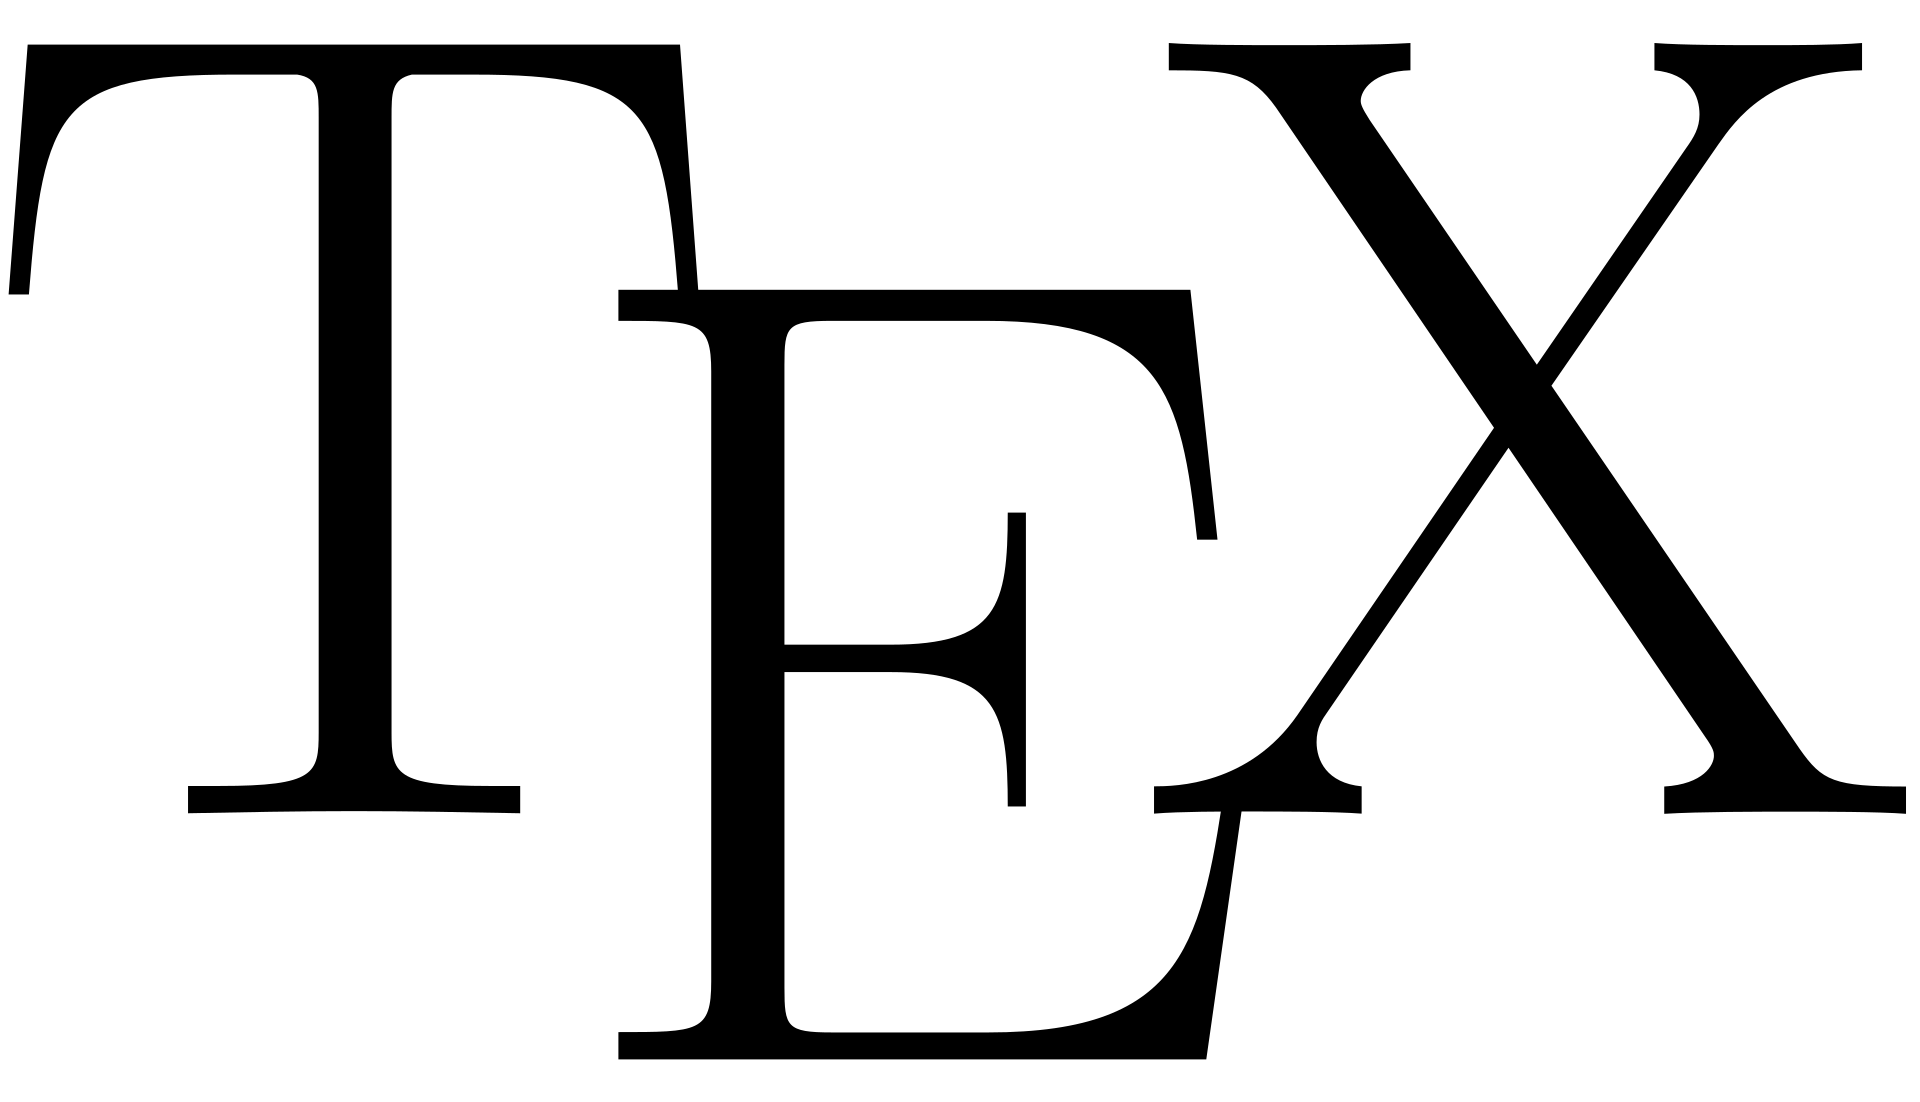
\includegraphics[width=0.2\linewidth]{TeX}
		\caption{Logo de TeX}
		\label{fig:subfig2}
	\end{subfigure}
	\caption{Ejemplo para poner dos figuras juntas. Y citarlas por separado a (\subref{fig:subfig1}) y (\subref{fig:subfig2}).}
	% OJO: el caption siempre va antes del label
	\label{fig:subfigs}
\end{figure}



% Para hacer que quede todo en una misma linea, se puede usar minipage
%\begin{minipage}[t]{\textwidth}
	\begin{lstlisting}[caption={Ejemplo de código (usando los estilos de la cátedra, ver las macros para más detalles)},label=code:for]
res := 0;
i := 0;
while (i < s.size()) do
	res := res + s[i];
	i := i + 1
endwhile
	\end{lstlisting}
%\end{minipage}

Si se pone un label al \verb|lstlisting|, se puede referenciar: Código \ref{code:for}.


\subsection{Macros de la cátedra para especificar}

\begin{proc}{nombre}{\In paramIn : \nat, \Inout paramInout : \TLista{\ent}}{tipoRes}
	%    \modifica{parametro1, parametro2,..}
	\requiere{expresionBooleana1}
	\asegura{expresionBooleana2}
	\aux{auxiliar1}{parametros}{tipoRes}{expresion}
	\pred{pred1}{parametros}{expresion} 
\end{proc}

\aux{auxiliarSuelto}{parametros}{tipoRes}{expresion}
% \paraTodo{variable}{tipo}{expresion}
% \existe{variable}{tipo}{expresion}
% Pueden tener [unalinea] para que no se divida en varias lineas
\pred{predSuelto}{parametros}{\paraTodo[unalinea]{variable}{tipo}{algo \implicaLuego expresion}}
\pred{predSuelto}{parametros}{\existe[unalinea]{variable}{tipo}{algo \yLuego expresion}}



\end{document}
